\documentclass{beamer}

%%% Обязательные пакеты
%% Beamer
\usepackage{beamerthemesplit}
\usetheme{SPbGU}
\beamertemplatenavigationsymbolsempty
\usepackage{appendixnumberbeamer}

%% Локализация
\usepackage{fontspec}
\setmainfont{CMU Serif}
\setsansfont{CMU Sans Serif}
\setmonofont{CMU Typewriter Text}
%\setmonofont{Fira Code}[Contextuals=Alternate,Scale=0.9]
%\setmonofont{Inconsolata}
% \newfontfamily\cyrillicfont{CMU Serif}

\usepackage{polyglossia}
\setdefaultlanguage{russian}
\setotherlanguage{english}
\usepackage[autostyle]{csquotes} % Правильные кавычки в зависимости от языка
\usepackage{framed}

%% Графика
\usepackage{wrapfig} % Позволяет вставлять графику, обтекаемую текстом
\usepackage{pdfpages} % Позволяет вставлять многостраничные pdf документы в текст

%% Математика
\usepackage{amsmath, amsfonts, amssymb, amsthm, mathtools} % "Адекватная" работа с математикой в LaTeX

% Математические окружения с русским названием
\newtheorem{rutheorem}{Теорема}
\newtheorem{ruproof}{Доказательство}
\newtheorem{rudefinition}{Определение}
\newtheorem{rulemma}{Лемма}

\newcommand\pro{\item[$+$]}
\newcommand\con{\item[$-$]}
\newcommand\emptyitem{\item[$$]}


%%% Дополнительные пакеты. Используются в презентации, но могут быть отключены при необходимости
\usepackage{tikz} % Мощный пакет для создание рисунков, однако может очень сильно замедлять компиляцию
\usetikzlibrary{decorations.pathreplacing,calc,shapes,positioning,tikzmark}

\usepackage{multirow} % Ячейка занимающая несколько строк в таблице

%% Пакеты для оформления алгоритмов на псевдокоде
\usepackage[noend]{algpseudocode}
\usepackage{algorithm}
\usepackage{algorithmicx}

\usepackage{fancyvrb}

% То, что в квадратных скобках, отображается внизу по центру каждого слайда. 
\title[BFS-based RPQ]{Алгоритм в терминах линейной алгебры для поиска путей от нескольких стартовых вершин с регулярными ограничениями}

% То, что в квадратных скобках, отображается в левом нижнем углу. 
\institute[СПбГУ]{}

% То, что в квадратных скобках, отображается в левом нижнем углу.
\author[Денис Порсев]{Порсев Денис Витальевич, 19.Б10-мм}
\date{9 июня 2023}
 
\begin{document}
{
\setbeamertemplate{footline}{}
\begin{frame}
  
\includegraphics[width=1.4cm]{pictures/SPbGU_Logo.png}
  \vspace{-45pt}
  \hspace{-10pt}
  \begin{center}
    \begin{tabular}{c}
      \scriptsize{Санкт-Петербургский государственный университет} \\
      \scriptsize{Математическое обеспечение и администрирование}  \\ \scriptsize{информационных систем}
    \end{tabular}
    \titlepage
  \end{center}

  \btVFill

  {\scriptsize
    \textbf{Научный руководитель:} доцент кафедры информатики, к.ф.-м.н., С.В. Григорьев\\
    \textbf{Рецензент:} эксперт ООО “Техкомпания Хуавэй” С.В. Моисеев
  }
  \begin{center}
    \vspace{5pt}
    \scriptsize{Санкт-Петербург\\
      2023}
  \end{center}

\end{frame}
}

\begin{frame}[fragile]
  \frametitle{Введение}
  \noindent\begin{minipage}{0.55\textwidth}
    \begin{itemize}
      \item Графовая модель данных
            \begin{itemize}
              \item Уникальный $Id$ вершины
              \item Вершины имеют свойства в формате ключ-значение
              \item Метка из $\mathcal{L}$ на каждом ребре
            \end{itemize}
      \item Применение:
            \begin{itemize}
              \item Анализ социальных сетей
              \item Биоинформатика
              \item Графовые базы данных (Redis~Graph, Neo4j)
            \end{itemize}
    \end{itemize}
  \end{minipage}
  \noindent\begin{minipage}{0.44\textwidth}
    \begin{figure}[h!]
      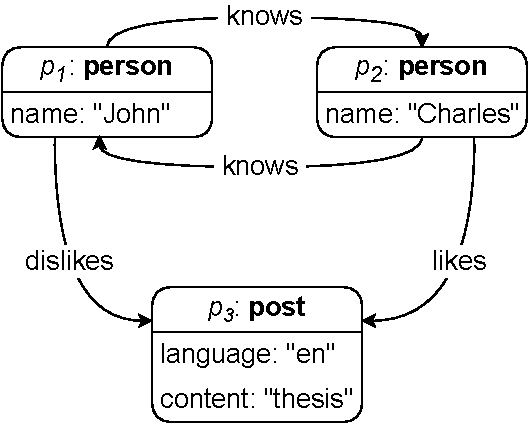
\includegraphics[width=1\linewidth]{pictures/graphmodel_intro.pdf}
      \caption*{$\mathcal{L}$: $\{knows, likes, dislikes\}$}
    \end{figure}
  \end{minipage}
\end{frame}

\begin{frame}[fragile]
  \frametitle{Поиск путей с регулярными ограничениями (RPQ)}
  \noindent\begin{minipage}{0.55\textwidth}
    \begin{itemize}
      \item Запрос к графовой БД
      \item Ограничения на пути в графе в виде регулярного языка
      \item \textit{Property paths} в SPARQL v1.1
            \vspace{2pt}
            \begin{itemize}
              \emptyitem $?person$ :$knows^*$ $?person$ .
              \emptyitem $?person$ $($:$knows/$:$likes)^+$ $?post$ .
            \end{itemize}
            \vspace{2pt}
      \item Частичная поддержка в Cypher (Neo4j)
            \vspace{2pt}
            \begin{itemize}
              \emptyitem $(person)$$-$$[$:$knows^*]$$-$$>$$(person)$
            \end{itemize}
            \vspace{2pt}
    \end{itemize}
  \end{minipage}
  \noindent\begin{minipage}{0.44\textwidth}
    \begin{figure}[h!]
      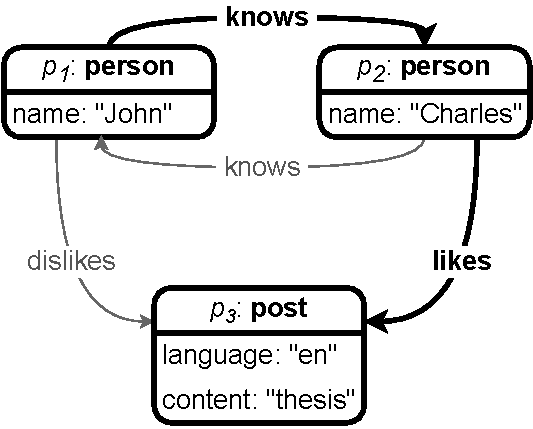
\includegraphics[width=1\linewidth]{pictures/graphmodel_path.pdf}
    \end{figure}
  \end{minipage}
\end{frame}


\begin{frame}[fragile]
  \frametitle{Разработанный ранее алгоритм (MSBFS)}
  \noindent\begin{minipage}{0.4\textwidth}
    \begin{itemize}
      \item Решает задачу RPQ
      \item Основан на матричном умножении
      \item Разреженные матрицы смежности
      \item BFS выражен в терминах линейной алгебры
      \item Реализован с помощью PyGraphBLAS\footnotemark
    \end{itemize}
  \end{minipage}
  \footnotetext{\href{https://pypi.org/project/pygraphblas/}{Обёртка} над библиотекой примитивных операций с разреженной лин. алгеброй SuiteSparse:GraphBLAS}
  \noindent\begin{minipage}{0.58\textwidth}
    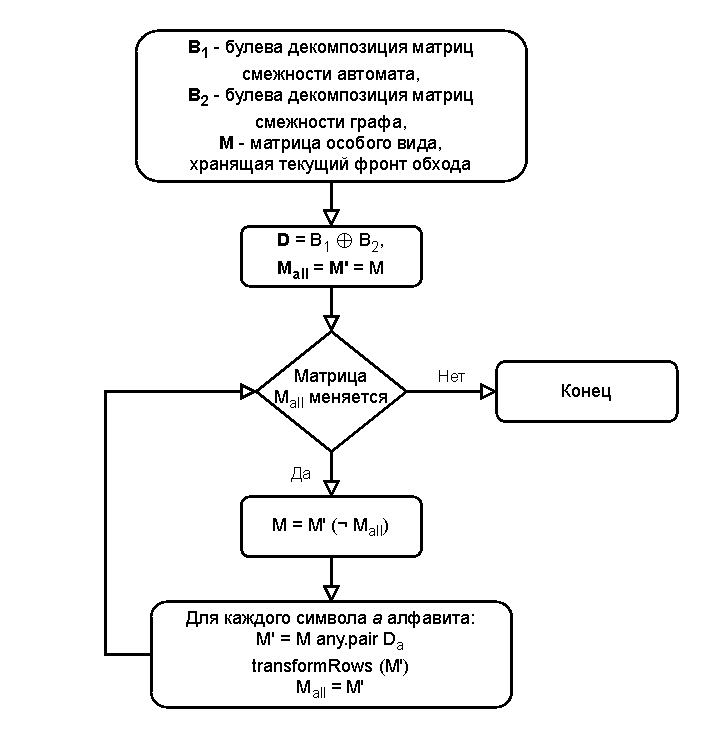
\includegraphics[width=1\linewidth]{pictures/algo.pdf}
  \end{minipage}
\end{frame}

\begin{frame}
  \frametitle{Постановка задачи}
  \textbf{Цель:} проведение экспериментального исследования алгоритма для решения задачи RPQ, основанного на поиске в ширину и выраженного в терминах линейной алгебры

  \textbf{Задачи:}
  \begin{itemize}
    \item Выбрать множество аналогов для проведения сравнения с ними
    \item Подготовить датасет, состоящий из графов и регулярных запросов
    \item Спроектировать инструмент автоматизации экспериментов
    \item Провести экспериментальное исследование алгоритмов и проанализировать результаты
  \end{itemize}
\end{frame}

\begin{frame}[fragile]
  \frametitle{Существующие решения задачи RPQ}
  \noindent\begin{minipage}{1\textwidth}
    \begin{itemize}
      \item Решения, основанные на использовании конечных автоматов и различных поисков (например, BFS)
      \item Datalog
            \begin{itemize}
              \pro Выразителен
              \pro Является стандартным бенчмарком для сравнения
              \con Необходимо самостоятельно реализовывать запросы с ограничениями в виде регулярных языков
            \end{itemize}
      \item Решения, строящие индекс по путям в графе
            \begin{itemize}
              \pro Получение результата за один просмотр индекса
              \con Большой расход памяти
            \end{itemize}
    \end{itemize}
  \end{minipage}
\end{frame}

\begin{frame}[fragile]
  \frametitle{Существующие решения задачи RPQ}
  \noindent\begin{minipage}{1\textwidth}
    \color{red}MSBFS
    \vspace{-9pt}
    \begin{itemize}
      \begin{framed}\color{black}
        \item Решения, основанные на использовании конечных автоматов и различных поисков (например, BFS)\color{red}
        \begin{itemize}
          \item Выразимы с помощью матричных операций
        \end{itemize}
      \end{framed}
      \color{black}
      \item Datalog
            \begin{itemize}
              \pro Выразителен
              \pro Является стандартным бенчмарком для сравнения
              \con Необходимо самостоятельно реализовывать запросы с ограничениями в виде регулярных языков
            \end{itemize}
      \item Решения, строящие индекс по путям в графе
            \begin{itemize}
              \pro Получение результата за один просмотр индекса
              \con Большой расход памяти
            \end{itemize}
    \end{itemize}
  \end{minipage}
\end{frame}

\begin{frame}[fragile]
  \frametitle{Выбор аналогов}
  \begin{itemize}
    \item Реализация тензорного алгоритма в репозитории CFPQ\_Pyalgo\footnote{\href{https://github.com/bahbyega/CFPQ_PyAlgo}{Репозиторий} для исследования алгоритмов поиска путей с ограничениями в виде формальных языков, реализованных на основе стандарта GraphBLAS}
          \begin{itemize}
            \item Представление запросов:
                  \begin{center}
                    $l^*$ $\Rightarrow$ $S \rightarrow l$ $S$ $|$ $\epsilon$
                  \end{center}
          \end{itemize}
    \item Souffle --- реализация Datalog, часто используемая в задачах языкового анализа и набирающая большую популярность
          \begin{itemize}
            \item Генерация программ Datalog:
                  \begin{center}
                    $l^*$\\
                    $\Downarrow$\\
                    $path(x, y) :$-- $edge(x, l, z), path(z, y).$\\
                    $path(x, y) :$-- $edge(x, l, y).$
                  \end{center}
                  \vspace{5pt}
          \end{itemize}
    \item Алгоритмы, строящие индексы, не вошли в сравнительный анализ
          \begin{itemize}
            \item Большинство встроены в системы баз данных
          \end{itemize}
  \end{itemize}

\end{frame}

\begin{frame}[fragile]
  \frametitle{Сбор данных: графы}
  Данные:
  \begin{itemize}
    \item RDF-графы
    \item Социальные сети
  \end{itemize}
  \vspace{10pt}
  \noindent\begin{minipage}{1\textwidth}
    \begin{table}[!ht]
      \centering
      \begin{tabular}{|c|c|c|c|}
        \hline
        Graph      & \#V       & \#E        & \#L \\ \hline \hline
        enzyme     & 48 815    & 86 543     & 14  \\
        eclass     & 239 111   & 360 248    & 10  \\
        go         & 582 929   & 1 437 437  & 47  \\
        geospecies & 450 609   & 2 201 532  & 158 \\
        taxonomy   & 5 728 398 & 14 922 125 & 21  \\
        \hline
        advogato   & 6 541     & 51 127     & 3   \\
        youtube    & 15 088    & 27 257 790 & 5   \\
        \hline
      \end{tabular}
    \end{table}
  \end{minipage}
  \noindent\begin{minipage}{0.25\textwidth}
  \end{minipage}
\end{frame}

\begin{frame}[fragile]
  \frametitle{Сбор данных: запросы}
  \begin{itemize}
    \item Набор из 16 популярных шаблонов для запросов
    \item Генерация запросов с самыми популярными метками
  \end{itemize}
  \vspace{10pt}
  \noindent\begin{minipage}{1
      \textwidth}
    \begin{table}[!ht]
      \centering
      \begin{tabular}{|c|c||c|c|}
        \hline
        Name  & Query                           & Name     & Query                                           \\ \hline \hline
        $q_0$ & $a^*$                           & $q_{8}$  & $a \cdot b$                                     \\
        $q_1$ & $a \cdot b^*$                   & $q_{9}$  & $a \cdot b \cdot c$                             \\
        $q_2$ & $a \cdot b^* \cdot c^*$         & $q_{10}$ & $a \cdot b \cdot c \cdot d$                     \\
        $q_3$ & $a \cdot b^* \cdot c$           & $q_{11}$ & $(a \cdot b)^+~|~(c \cdot d)^+$                 \\
        $q_4$ & $a^* \cdot b^*$                 & $q_{12}$ & $(a \cdot (b \cdot c)^*)^+~|~(d \cdot e)^+$     \\
        $q_5$ & $a \cdot b \cdot c^*$           & $q_{13}$ & $(a \cdot b \cdot (c \cdot d)^*)^+~|~(e~|~f)^*$ \\
        $q_6$ & $(a~|~b~|~c~|~d~|~e)^+$         & $q_{14}$ & $(a~|~b)^+ (c~|~d)^+$                           \\
        $q_7$ & $(a~|~b~|~c~|~d~|~e) \cdot f^*$ & $q_{15}$ & $a \cdot b \cdot (c~|~d~|~e)$                   \\
        \hline
      \end{tabular}
    \end{table}
  \end{minipage}
  \noindent\begin{minipage}{0.25\textwidth}
  \end{minipage}
\end{frame}

\begin{frame}[fragile]
  \frametitle{Инструмент для автоматизации экспериментов}
  \begin{center}
    \begin{minipage}{0.9\textwidth}
      \begin{figure}[h!]
        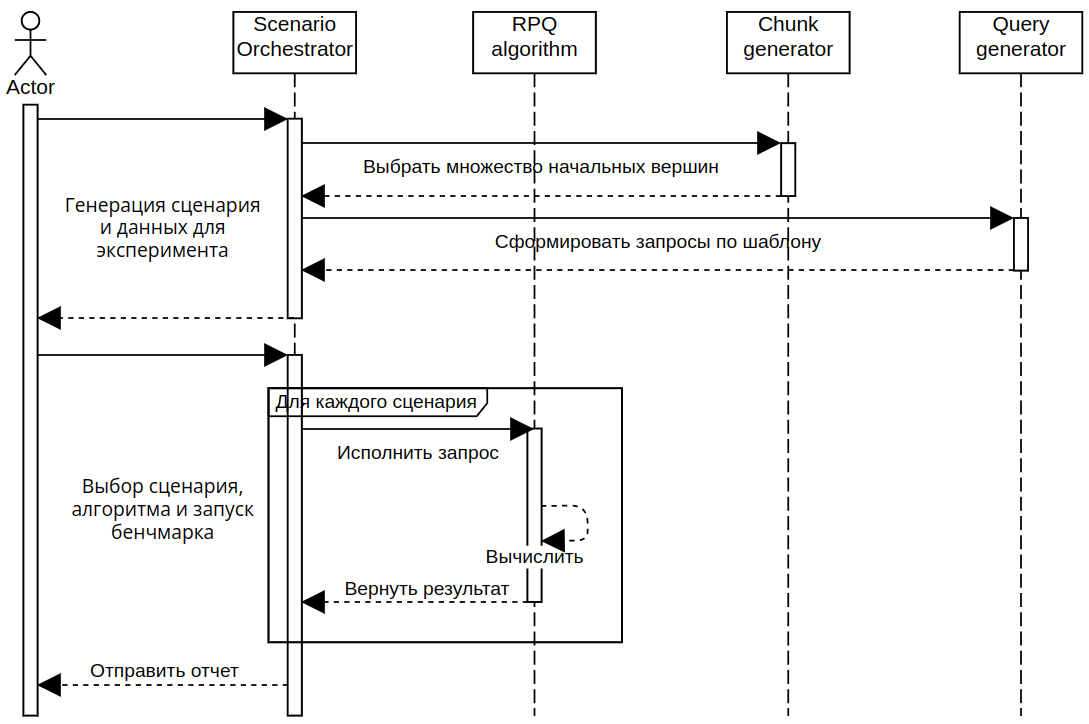
\includegraphics[width=1\linewidth]{pictures/arch.png}
      \end{figure}
    \end{minipage}
  \end{center}
\end{frame}

\begin{frame}[fragile]
  \frametitle{Экспериментальное исследование}
  Конфигурация:
  \begin{itemize}
    \item Ubuntu 20.04, процессор Intel i7-4790 CPU @ 3.60GHz CPU, оперативная память DDR4 64 Gb
  \end{itemize}
  \vspace{10pt}
  Исследовательские вопросы:
  {
  \begin{itemize}
    \item[\textbf{В1:}] Какова производительность разработанного алгоритма по сравнению с существующими аналогами?

    \item[\textbf{В2:}] Как влияет размер множества стартовых вершин на производительность реализации разработанного алгоритма?
  \end{itemize}
  }
\end{frame}

\begin{frame}[fragile]
  \frametitle{B1: Single--source запросы}
  \begin{figure}
    \begin{tabular}{cc}
      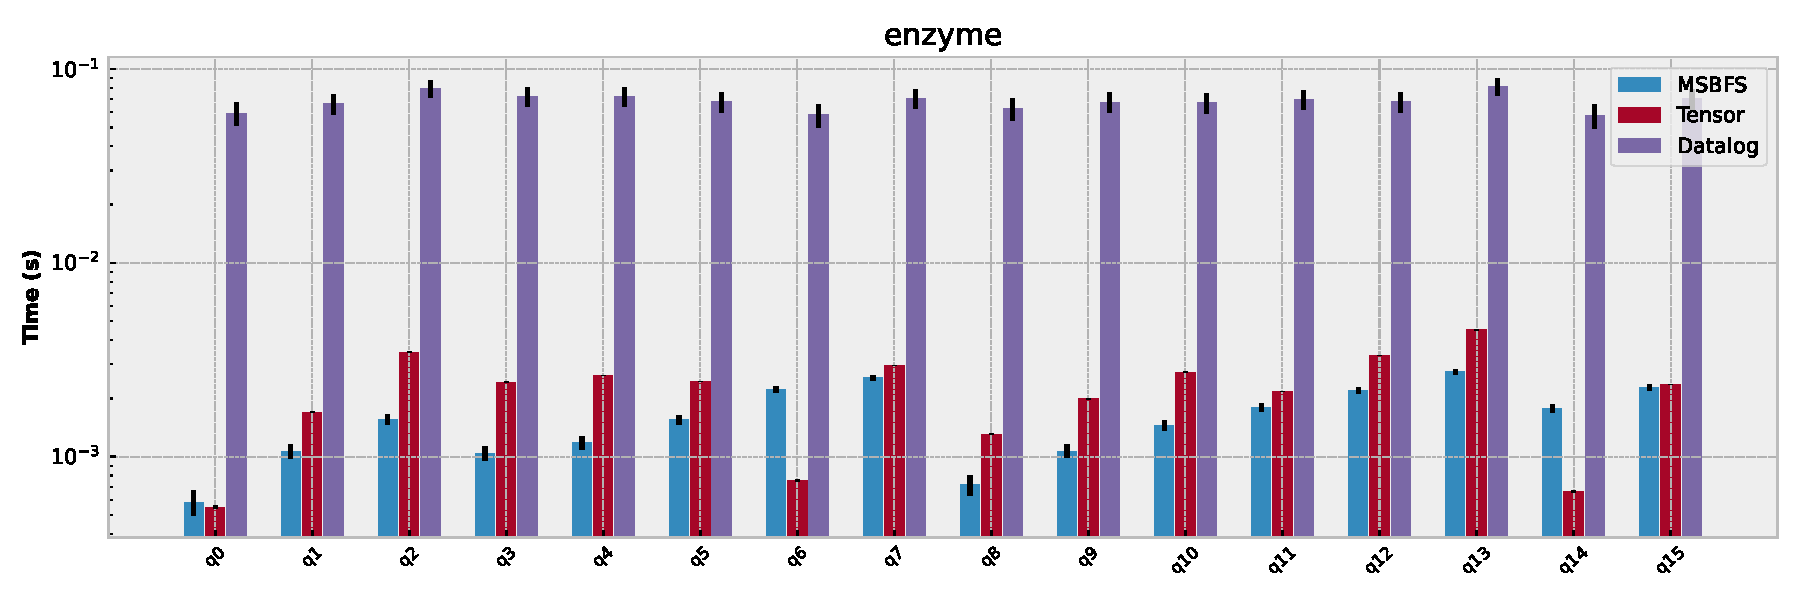
\includegraphics[width=110mm]{pictures/enzyme_ss.pdf}     \\
      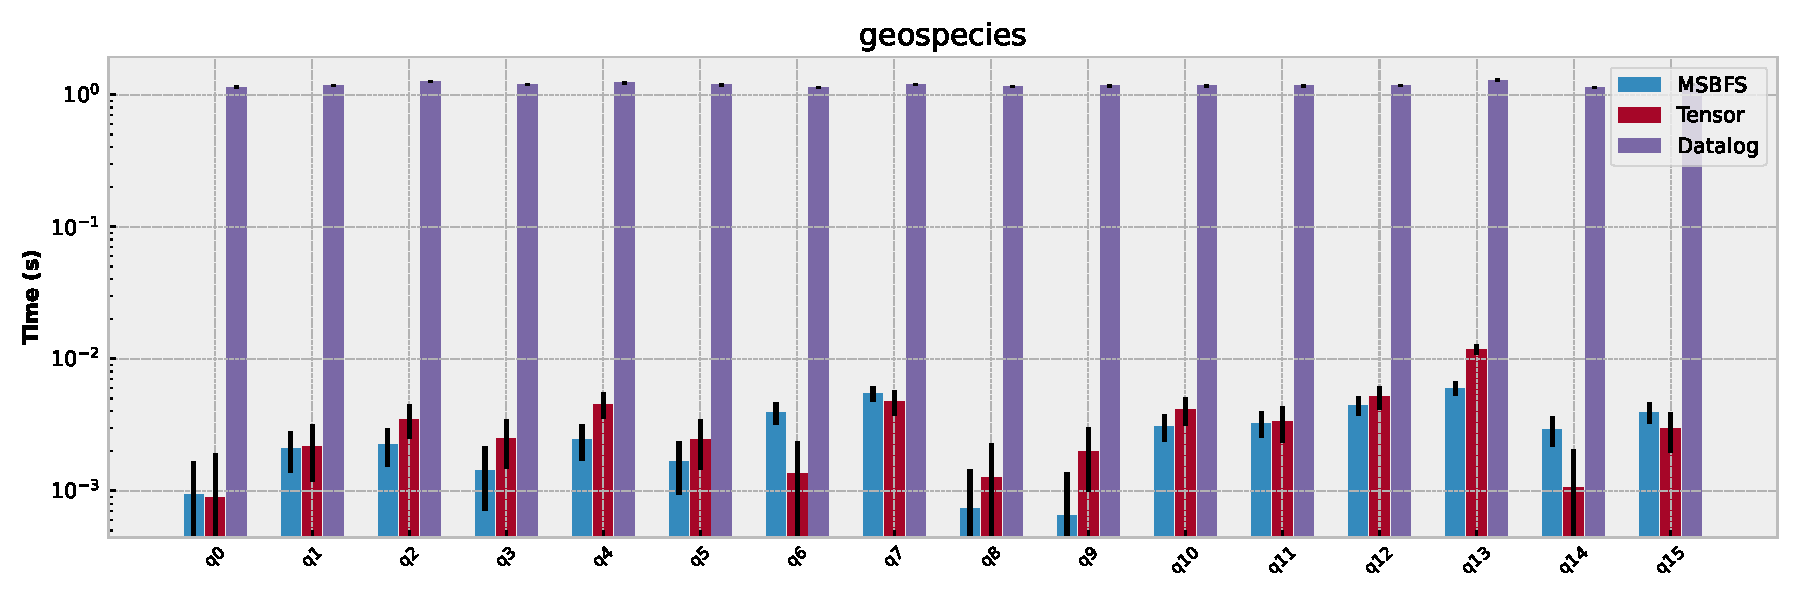
\includegraphics[width=110mm]{pictures/geospecies_ss.pdf} \\
    \end{tabular}
  \end{figure}
\end{frame}

\begin{frame}[fragile]
  \frametitle{B1: Multiple-source запросы (10 000 стартовых вершин)}
  \begin{figure}
    \begin{tabular}{cc}
      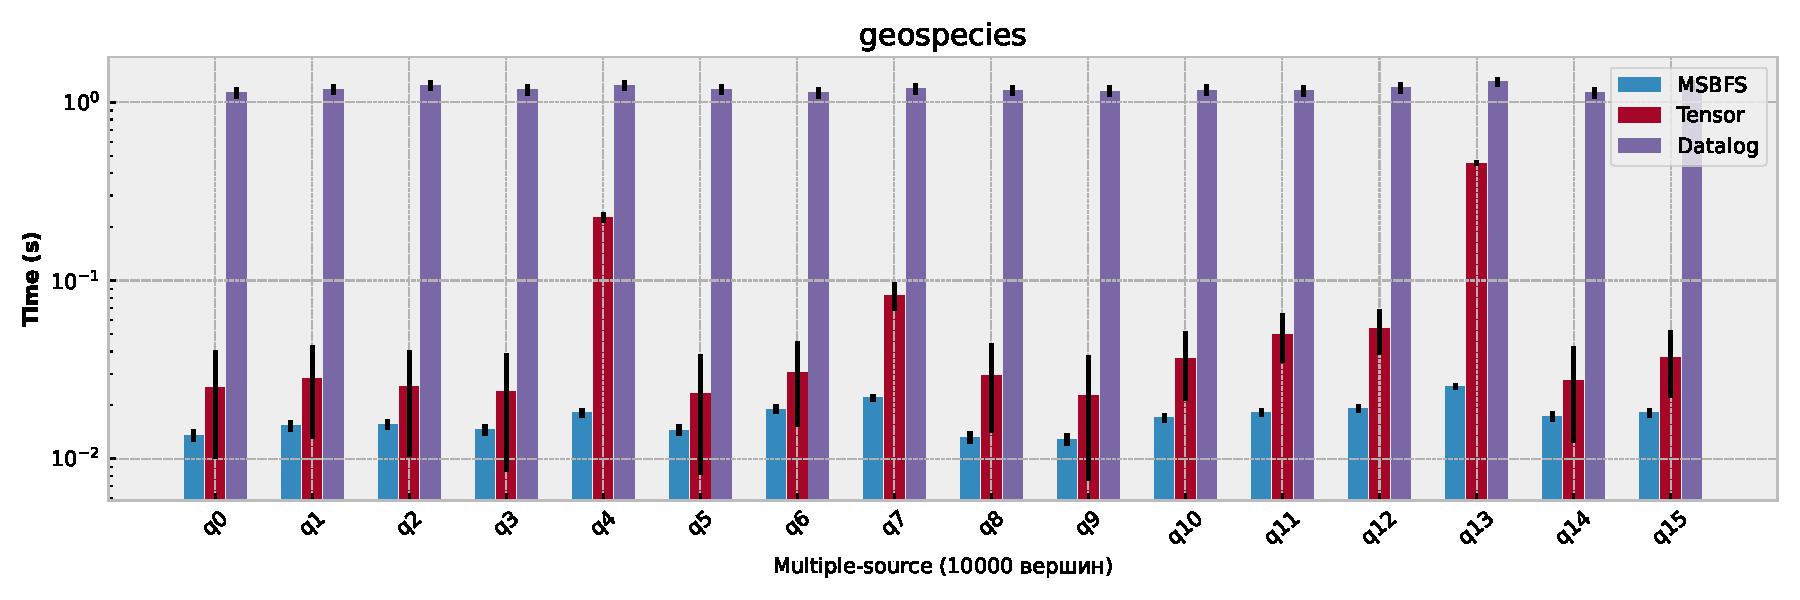
\includegraphics[width=110mm]{pictures/geospecies_10000.pdf} \\
      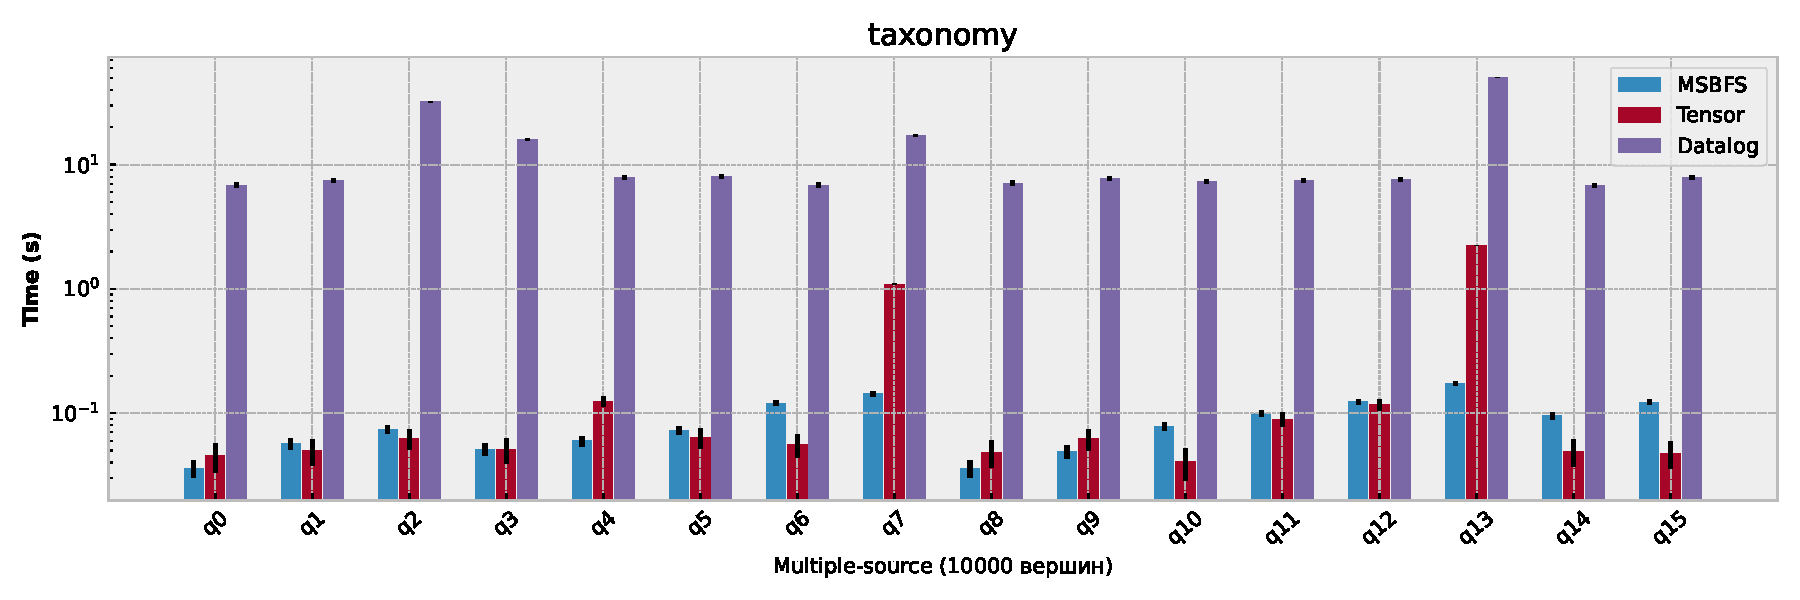
\includegraphics[width=110mm]{pictures/taxonomy_ms10000.pdf} \\
    \end{tabular}
  \end{figure}
\end{frame}

\begin{frame}[fragile]
  \frametitle{B2: постановка эксперимента}
  \begin{itemize}
    \item Число стартовых вершин: 1, 2, 5, 10, 100, 1000, 10000
    \item Две реализации MSBFS:
          \begin{itemize}
            \item MSBFS находит множество достижимых вершин
            \item MSBFSPairs находит множество достижимых вершин для каждой стартовой вершины
          \end{itemize}
    \item Сравнение с тензорным алгоритмом
    \item Взяты самые большие RDF графы + графы социальных сетей
  \end{itemize}
\end{frame}

\begin{frame}[fragile]
  \frametitle{B2: Размер множества стартовых вершин}
  \begin{figure}
    \begin{tabular}{cc}
      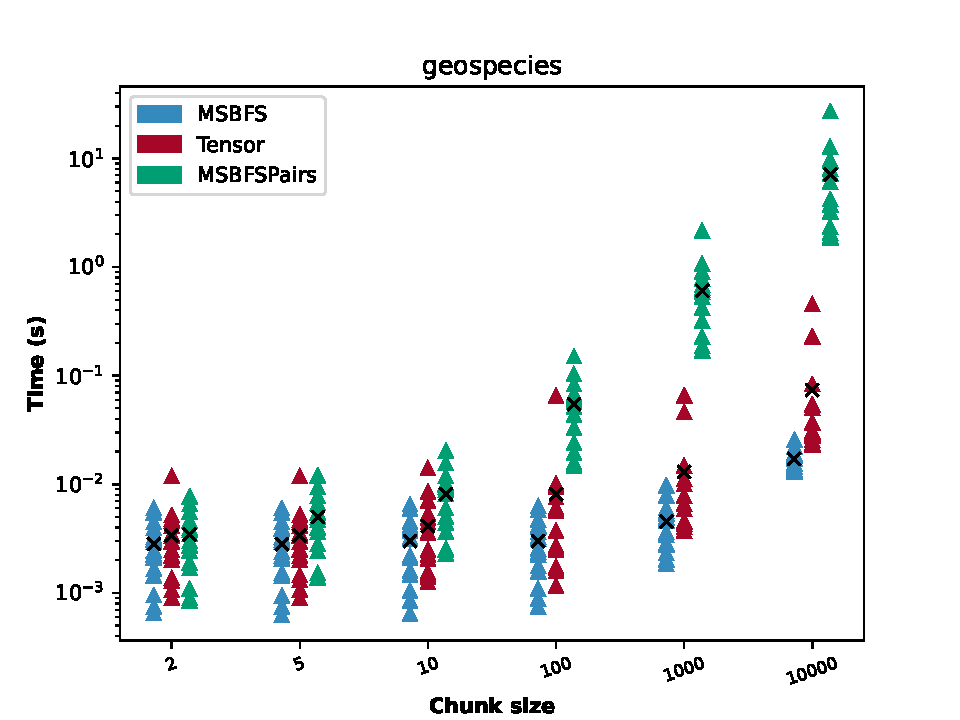
\includegraphics[width=50mm]{pictures/chunks-geospecies.pdf} & 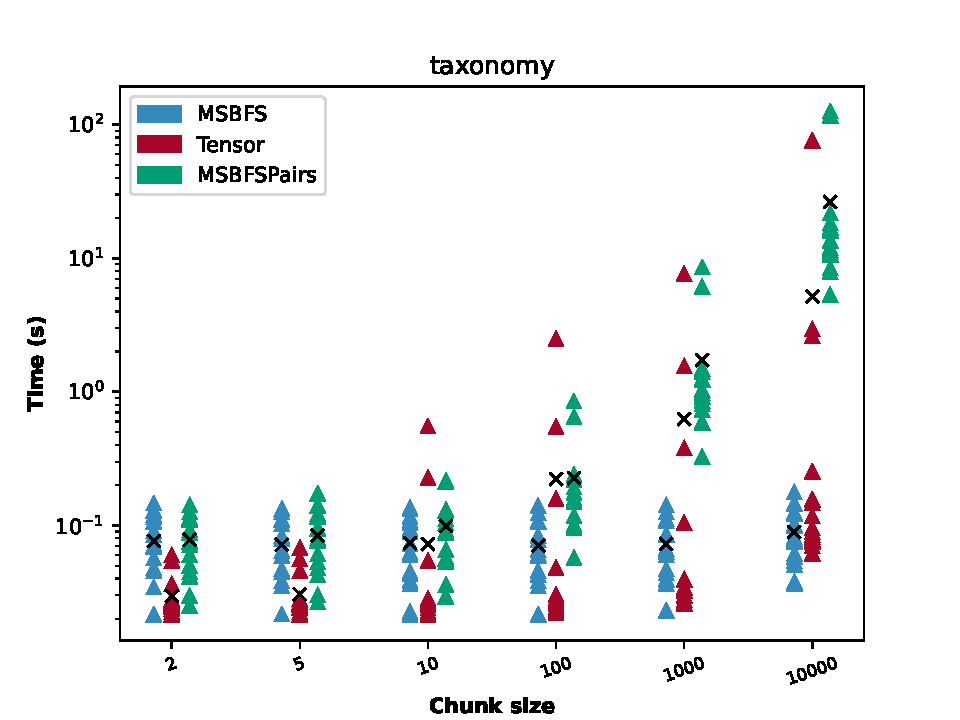
\includegraphics[width=50mm]{pictures/chunks-taxonomy.pdf} \\
      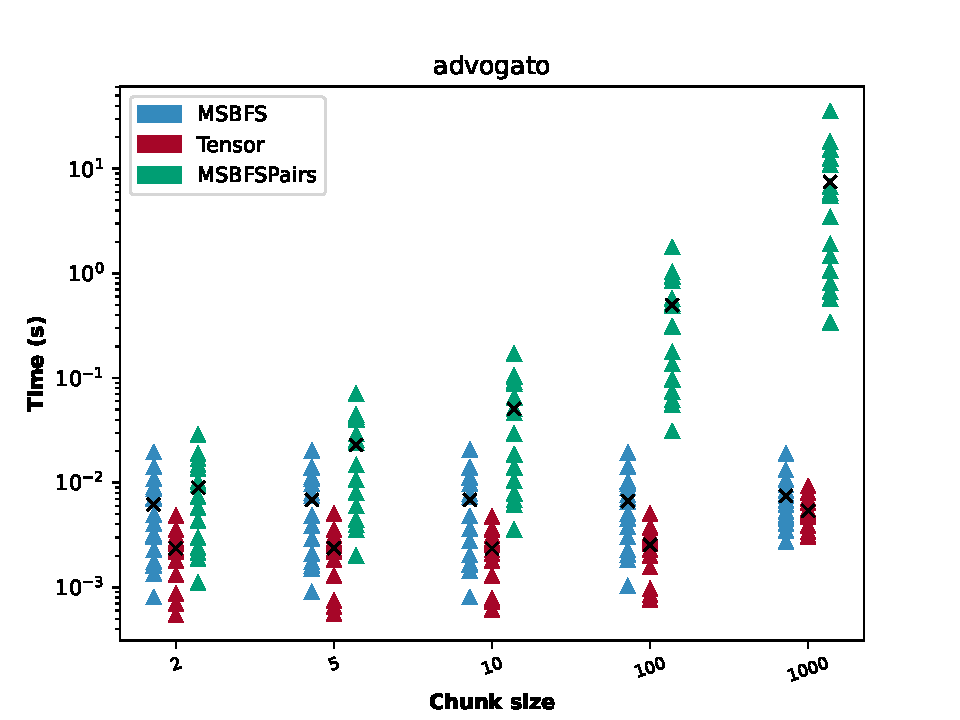
\includegraphics[width=50mm]{pictures/chunks-advogato.pdf}   & 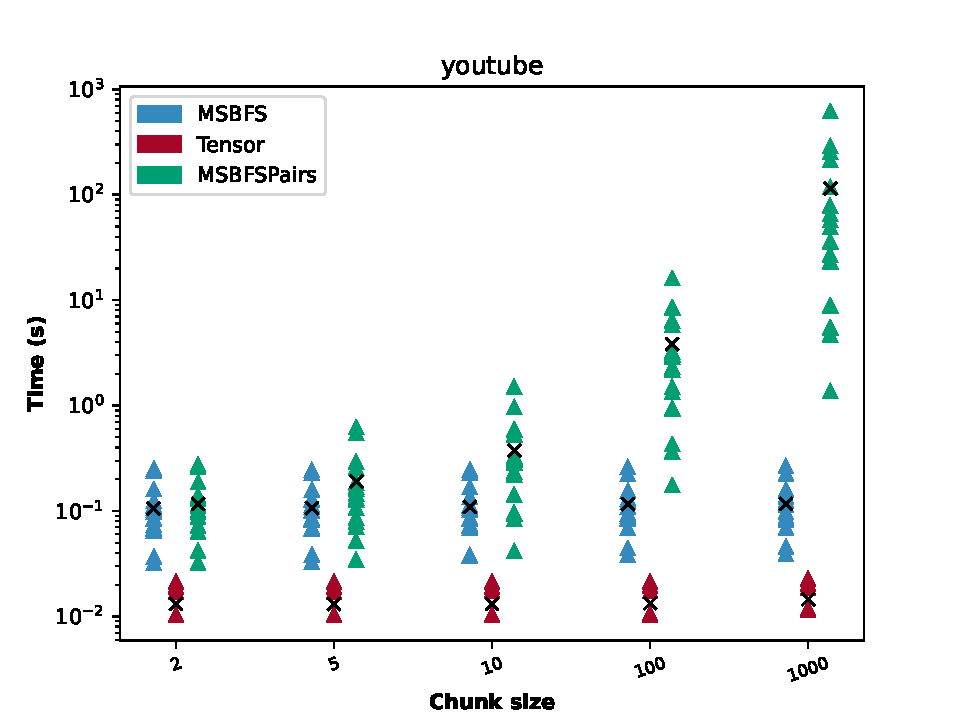
\includegraphics[width=50mm]{pictures/chunks-youtube.pdf}  \\
    \end{tabular}
  \end{figure}
\end{frame}

\begin{frame}
  \frametitle{Результаты}
  \begin{itemize}
    \item Проведен обзор и выбрано два аналога для сравнения: тензорный алгоритм, Datalog (Souffle)
    \item Собран датасет из графов и регулярных запросов
    \item Разработан инструмент\footnote{\href{https://github.com/bahbyega/paths-benchmark}{https://github.com/bahbyega/paths-benchmark}} для автоматизации экспериментов
    \item Проведено экспериментальное исследование нового алгоритма:
          \begin{itemize}
            \item Алгоритм MSBFS показывает приемлемое время работы, опережает Datalog
            \item На графах RDF алгоритм MSBFS в среднем более производителен аналогов, на графах социальных сетей тензорный алгоритм оказался самым быстрым
            \item При увеличении числа стартовых вершин несущественное падение производительности реализации MSBFS множество-множество; для MSBFSPairs наблюдается сильный рост времени исполнения
          \end{itemize}
  \end{itemize}
\end{frame}

\appendix

\begin{frame}[fragile]
  \frametitle{Дополнительно B1: Multiple-source запросы (1 000)}
  \begin{figure}
    \begin{tabular}{cc}
      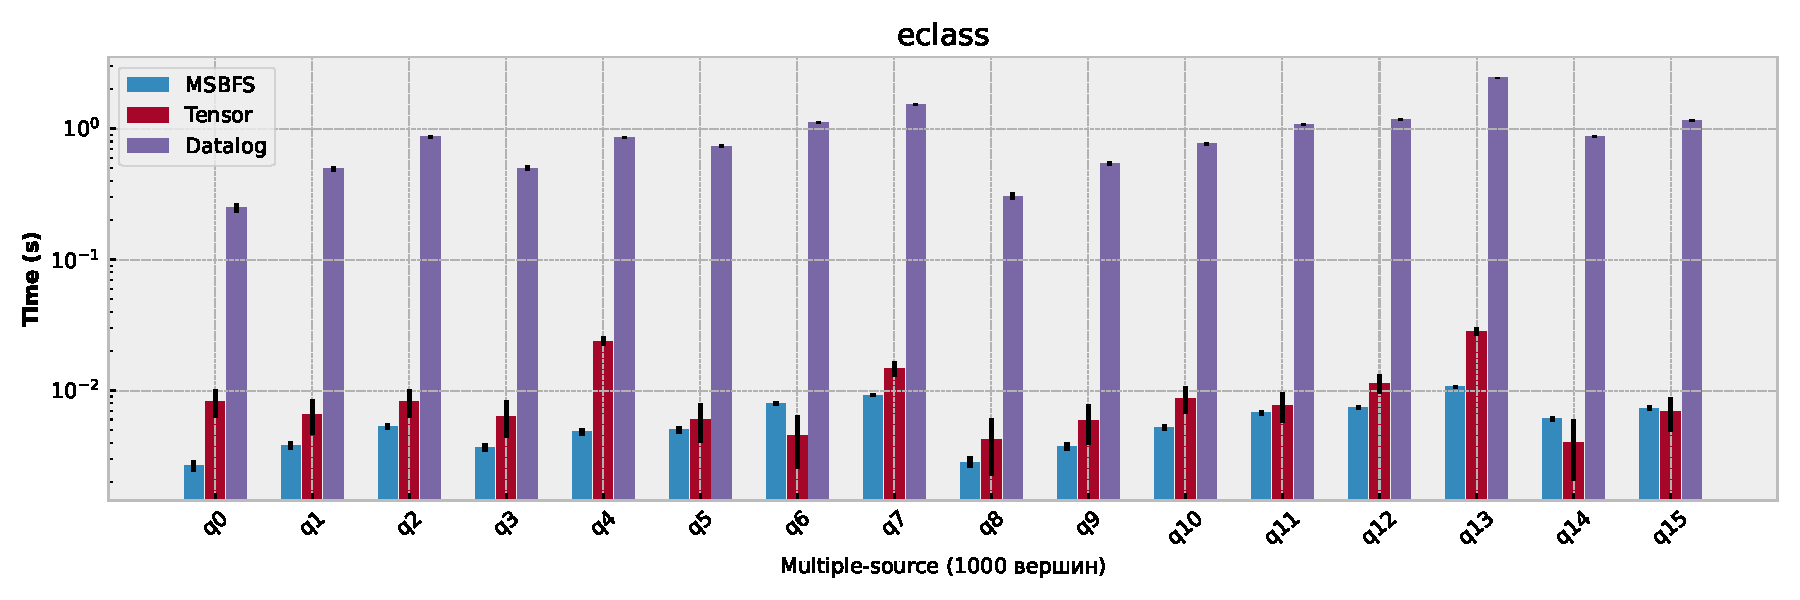
\includegraphics[width=110mm]{pictures/eclass_ms1000.pdf}     \\
      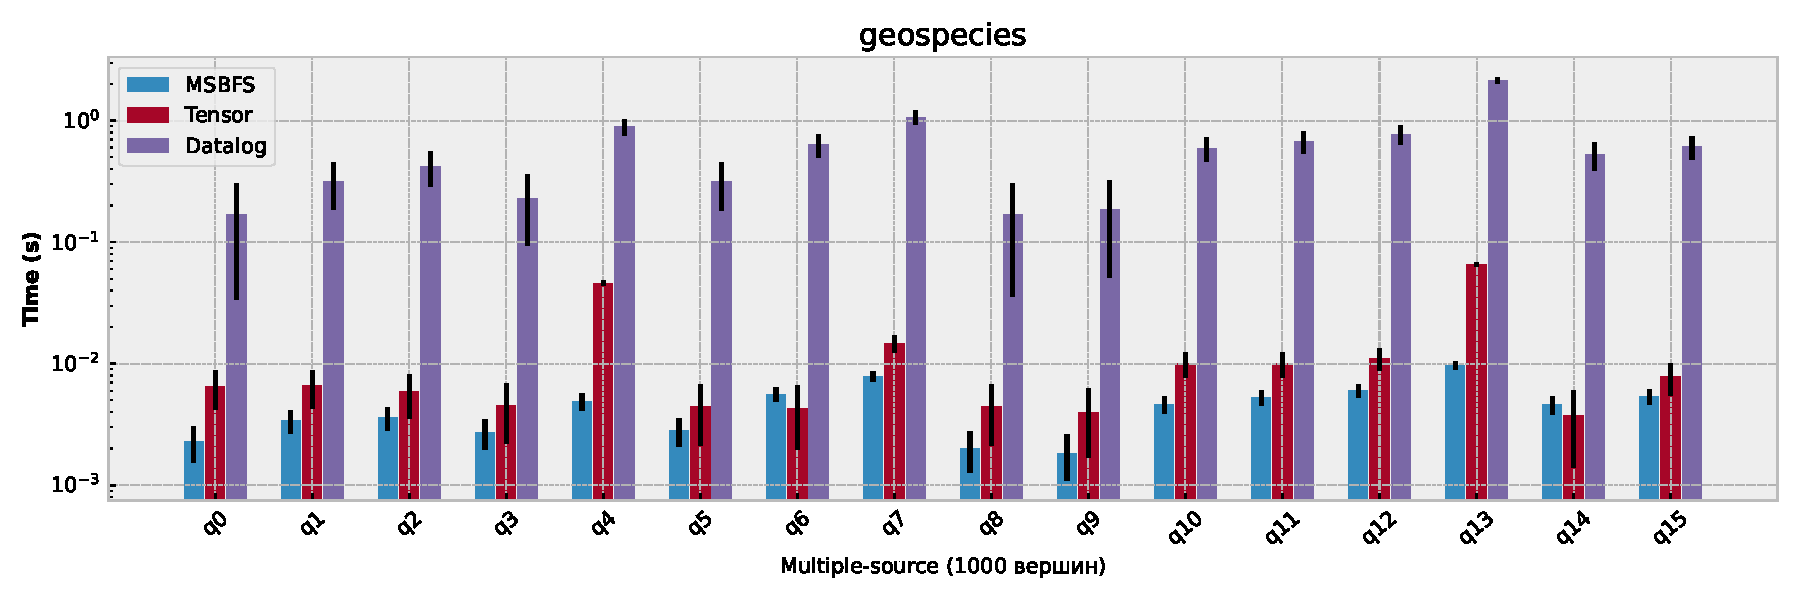
\includegraphics[width=110mm]{pictures/geospecies_ms1000.pdf} \\
    \end{tabular}
  \end{figure}
\end{frame}

\begin{frame}[fragile]
  \frametitle{Дополнительно: Алгоритм в псевдокоде}
  \begin{figure}
    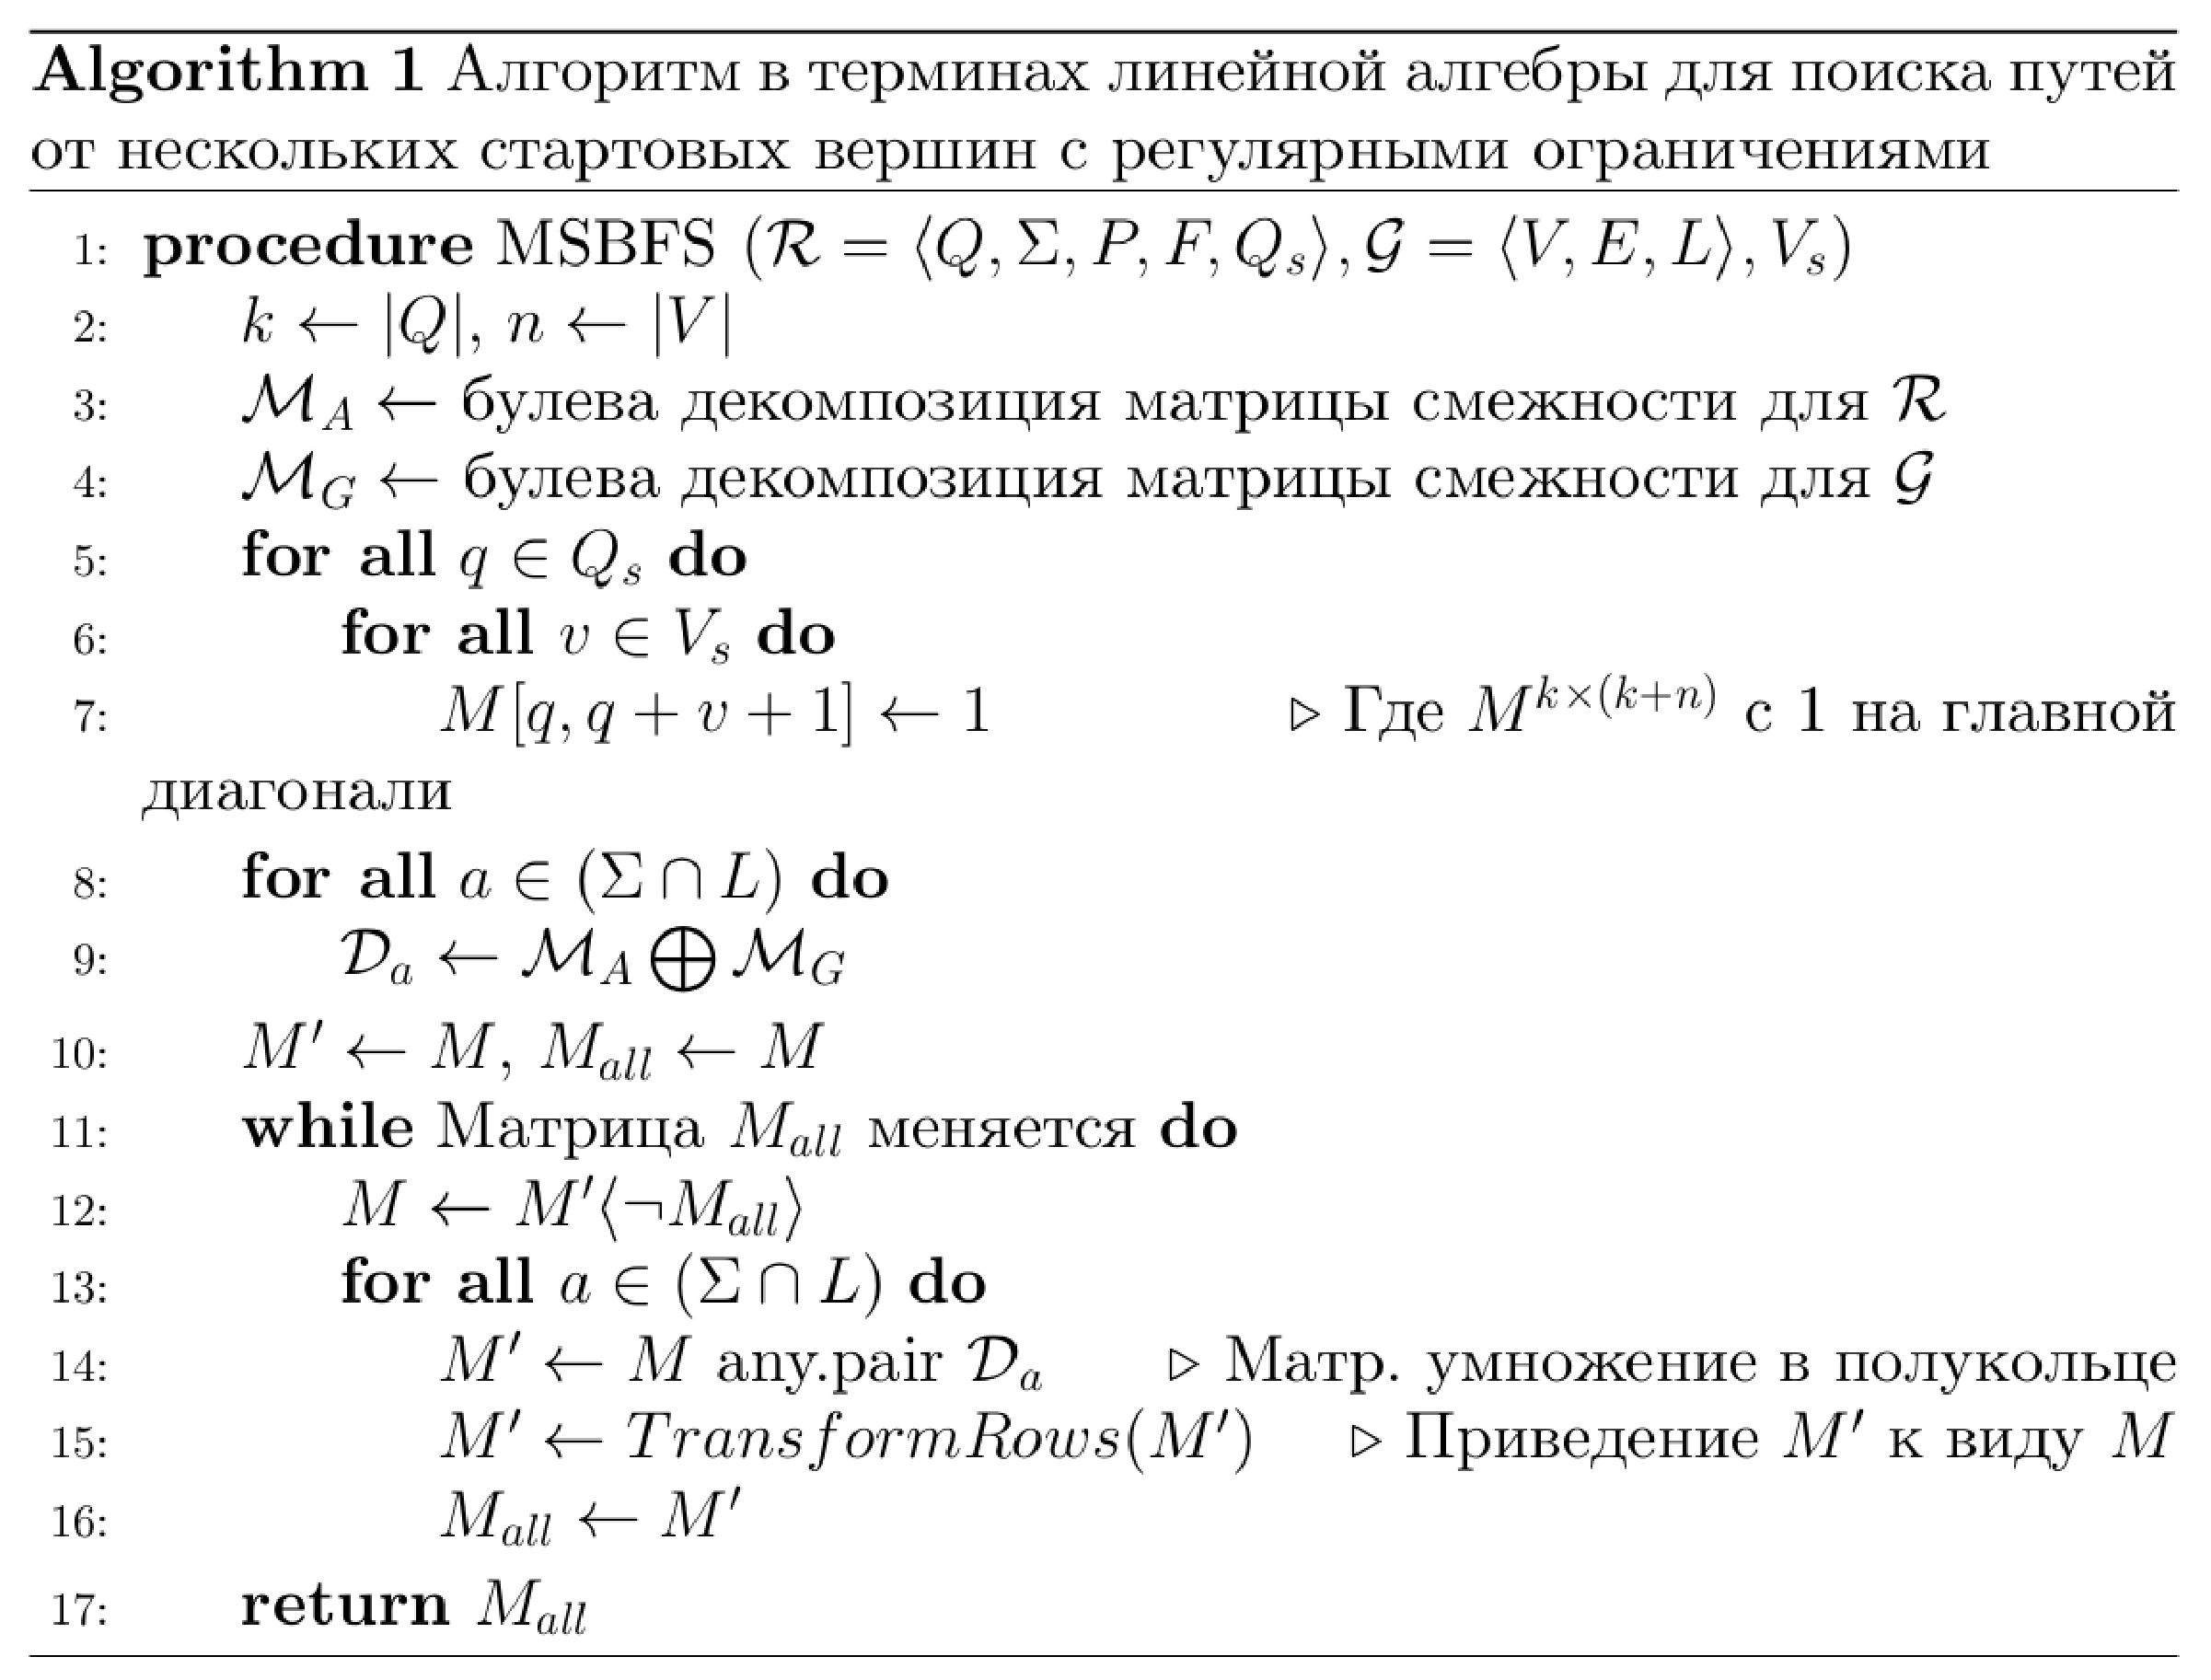
\includegraphics[width=0.85\linewidth]{pictures/algo_pseudo.pdf}\\
  \end{figure}
\end{frame}

\end{document}